\documentclass{article}
\usepackage[ngerman]{babel}
\usepackage[utf8]{inputenc}
\usepackage{graphicx} 
\usepackage{svg}
\graphicspath{{Bilder/}}
\usepackage{geometry}
\usepackage{pdflscape}
\geometry{a4paper, top=25mm, left=30mm, right=25mm, bottom=20mm}
\begin{document}


\section*{Softwareentwurf}
Die Aufgaben der Software besteht darin, die Steuerung des Systems und die Kommunikation mit einer Bedieneinheit zu übernehmen. Als Plattform wird ein STM32F4-Discovery Board mit einem Free-RTOS Betriebssystem verwendet. In den folgenden Abschnitten werden die Aufgaben in Teilfunktion untergliedert und deren Implementation erörtert.

\section{Namen- und Typkonventionen}
Um einen einheitlichen Programmentwurf zu gewährleisten werden Konventionen zur Wahl von Bezeichnern festgelegt. In der Datei "Global.h"  werden die Bezeichnungen für Standarddatentypen definiert. In dieser Anwendung sind vorzugsweise vorzeichenlose Ganzzahlen zu verwenden, vorzeichenbehaftete Ganz- und Gleitpunktzahlen sind nur in zwingend erforderlichen Situation, wie z.B. Berechnung der Reglerwerte, zu verwenden. Hierbei ist besondere Sorgfalt bei der Umrechnung zwischen den Datentypen erforderlich.

\begin{itemize} 
\item UInt8 : Vorzeichenlose Ganzzahl, 8Bit
\item UInt16 : Vorzeichenlose Ganzzahl, 16Bit
\item UInt32 : Vorzeichenlose Ganzzahl, 32Bit
\item UInt64 : Vorzeichenlose Ganzzahl, 64Bit
\item Int8 	: Vorzeichenbehaftete Ganzzahl, 8Bit
\item Int16 : Vorzeichenbehaftete Ganzzahl, 16Bit
\item Int32 : Vorzeichenbehaftete Ganzzahl, 32Bit
\item Int64 : Vorzeichenbehaftete Ganzzahl, 64Bit
\end{itemize}


Die folgenden Präfixe werden für Bezeichner verwendet.

\begin{itemize}
\item E : Enumeration
\item C	: Klasse
\item A	: Abstrakte Klasse
\item I	: Interface Klasse
\item T	: Template Klasse
\item S	: Klasse nach Singletonmuster
\item m	: Membervariable einer Klasse
\item s	: Statische Memebervariable einer Klasse
\end{itemize}

\section{Interruptverarbeitung}
Bei der Gestaltung von Interrupt-Service-Routinen muss Wert daraufgelegt werden kurze Funktionen zu entwerfen. D.h., dass bei Auftreten eines Interrupt die Quelle ausgewertet und daraufhin ggf. eine Nachricht erzeugt wird um das System über das Ereignis zu informieren. Alle Interruptquellen verwenden die selbe Prioritätsstufe\footnote{Eine Ausnahme bilden Prozessor-Faults (z.B. Memory-Bus-Fault), diese besitzen die höchste Interruptpriorität, welche für derartige Faults reserviert ist.}.

\newpage

\section{Komponentenarchitektur}
Einzelne Funktionen, welche parallel zu bearbeiten sind, werden als Komponenten implementiert. In diesem Projekt wird einerseits eine Komponente zur Steuerung des Systems und andererseits eine Kommunikationskomponente eingesetzt. Beide Komponenten werden in einem separaten Task ausgeführt. 
Die Kommunikation der Komponenten erfolgt über ein Nachrichtensystem. Um Nachrichten entgegenzunehmen wird jede Komponente mit einer Nachrichtenschlange ausgestattet. FreeRTOS stellt hierfür threadsafe Queues zur Verfügung.
Die Ausführung einer Komponente erfolgt mittels der \textit{run}-Methode, diese wird in dem jeweiligen Task aufgerufen. Diese Grundstruktur der Komponenten wird in der abstrakten Klasse \textit{AComponentBase} umgesetzt. Von dieser Basisklasse werden wiederum die konkreten Klassen \textit{SControlComponent} und \textit{SCommComponent} abgeleitet. Diese werden nach dem Singleton-Muster implementiert.

\begin{figure}[h]
	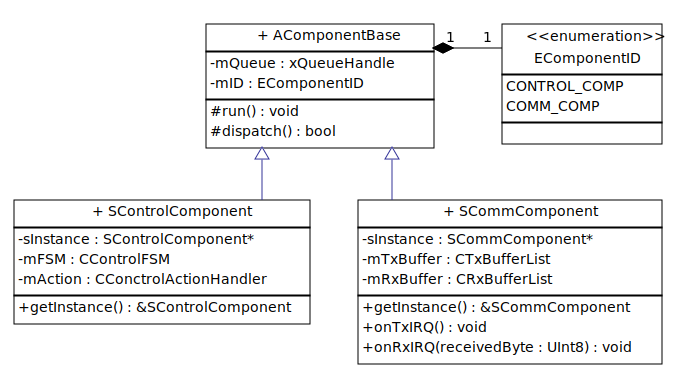
\includegraphics[width=\linewidth]{Komponentenarchitektur}
	\caption{Klassendiagramm Komponentenarchitektur, Quelle: eigene Darstellung}
\end{figure}

\newpage
\section{Kommunikation mittels Nachrichten}
Mit Hilfe von Nachrichten können die beiden Komponenten Informationen untereinander austauschen. Eine Nachricht enthält Informationen über den Sender, Empfänger und das Ereignis, welches die Nachricht veranlasst. Die Umsetzung der Nachrichten erfolgt in Form der Klasse \textit{CMessage}. An Hand des Nachrichten Typ in \textit{mType} kann das Event und somit der Nachrichteninhalt in \textit{mData} interpretiert werden.

\begin{figure}[h]
	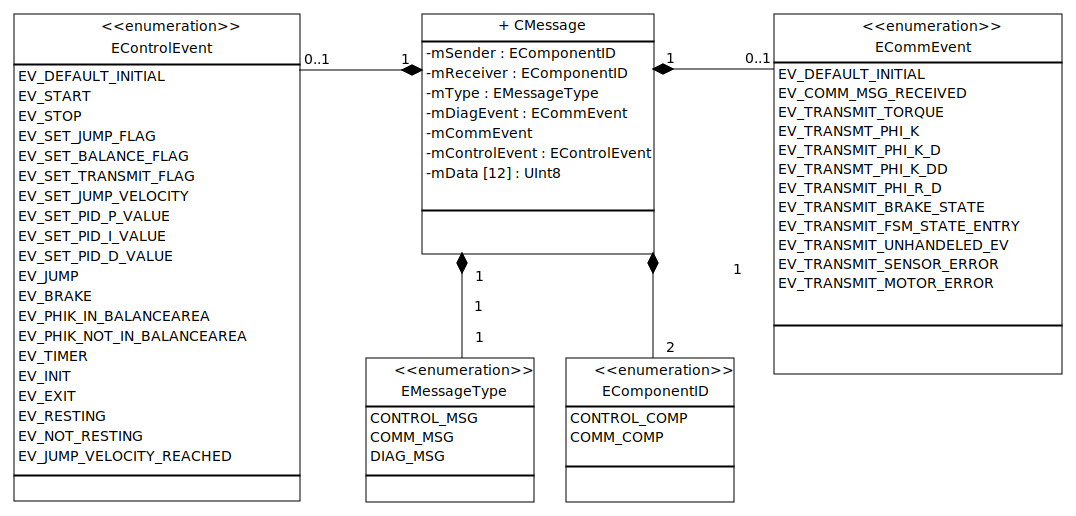
\includegraphics[width=\linewidth]{Nachrichtenstruktur}
	\caption{Klassendiagramm Nachrichtenstruktur, Quelle: eigene Darstellung}
\end{figure}

\subsection{Erzeugen und Verteilen der Nachrichten}
Die Nachrichten werden von der Klasse \textit{SProxy} erzeugt. Diese wird nach dem Singleton-Muster implementiert und dient als globale, öffentliche Schnittstelle zu den Komponenten. Auf Grund der überschaubaren Komponentenarchitektur übernimmt diese Einheit auch die Verteilung der Nachrichten. Hierfür ist keine dynamische Registrierung der Komponenten erforderlich, da die statische Verteilungshirachie vor Laufzeit feststeht.

\begin{figure}[h]
	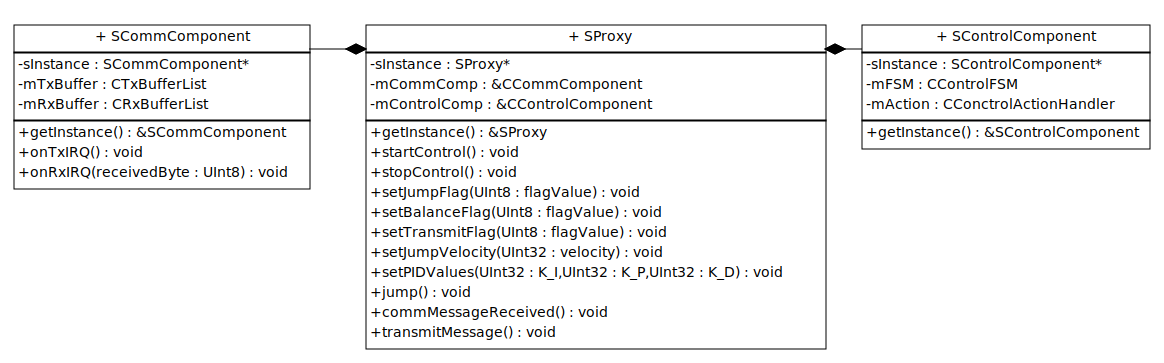
\includegraphics[width=\linewidth]{Proxy}
	\caption{Klassendiagramm Proxy, Quelle: eigene Darstellung}
\end{figure}

\newpage
\section{Aufbau der Kontrollkomponente}
Die Aufgabe der Kontrollkomponente besteht darin, den Würfel aufzurichten und in der gewünschten Gleichgewichtslage zu balancieren. Hierfür müssen die Sensoren ausgewertet und die Motoren entsprechend angesteuert werden. Die Regelungseinheit muss eine Schnittstelle bieten um die Parameter über die Bedieneinheit zu konfigurieren. Außerdem sollen die aktuellen Werte an die Bedieneinheit übermittelt werden.
Diese Funktionen werden in Form eines Zustandsautomaten implementiert. Mit Hilfe von Events können die gewünschten Funktionen aufgerufen werden.Die Ereignisse werden als Enumeration kodiert.
\begin{table}[h]
\centering
\label{my-label}
\begin{tabular}{|l|l|l|ll}
\cline{1-3}
\textbf{Eventkodierung}             & \textbf{Parameter} & \textbf{Kommentar}                                                                                                   &  &  \\ \cline{1-3}
EV\_START                  &                       & Startet die Steuerung                                                                                       &  &  \\ \cline{1-3}
EV\_STOP                   &                       & Stoppt die Steuerung                                                                                        &  &  \\ \cline{1-3}
EV\_SET\_JUMP\_FLAG        & FlagValue             & Setzt den Wert des JumpFlag                                                                                 &  &  \\ \cline{1-3}
EV\_SET\_BALANCE\_FLAG     & FlagValue             & Setzt den Wert des BalanceFlag                                                                              &  &  \\ \cline{1-3}
EV\_SET\_TRANSMIT\_FLAG    & FlagValue             & Setzt den Wert des TransmitFlag                                                                             &  &  \\ \cline{1-3}
EV\_SET\_JUMP\_VELOCITY    & VelocityValue         & \begin{tabular}[c]{@{}l@{}}Setzt die Geschwindigkeit der Schwung- \\masse zum 			Aufspringen\end{tabular}     &  &  \\ \cline{1-3}
EV\_SET\_PID\_VALUES       & K\_I, K\_P, K\_D      & Setzt Verstärkungsfaktoren des Regler                                                                       &  &  \\ \cline{1-3}
EV\_JUMP                   &                       & Leitet das Aufspringen ein                                                                                  &  &  \\ \cline{1-3}
EV\_TIMER                  &                       & Timerevent, realisiert Abtastzeit                                                                           &  &  \\ \cline{1-3}
EV\_BRAKE                  &                       & \begin{tabular}[c]{@{}l@{}}Internes Event, informiert über \\Betätigung 			der Bremse\end{tabular}          &  &  \\ \cline{1-3}
EV\_PHIK\_IN\_BAL\_EAREA  &                       & \begin{tabular}[c]{@{}l@{}}Internes Event, informiert über be- \\treten des 			Regelungsbereich\end{tabular}  &  &  \\ \cline{1-3}
EV\_PHIK\_NOT\_BAL\_AREA &                       & \begin{tabular}[c]{@{}l@{}}Internes Event, informiert über ver- \\lassen des 			Regelungsbereich\end{tabular} &  &  \\ \cline{1-3}
EV\_RESTING                &                       & Internes Event, Würfel in Ruheposition                                                                      &  &  \\ \cline{1-3}
EV\_NOT\_RESTING           &                       & Internes Event, Würfel nicht in Ruhe                                                                        &  &  \\ \cline{1-3}
EV\_VELOCITY\_REACHED  &                       & Internes Event, bereit zum Aufspringen                                                                      &  &  \\ \cline{1-3}
\end{tabular}
\end{table}

Der Zustandsautomat enthält die beiden Zustände \textit{CStateConfiguration} und \textit{CStateRunning}. In dem Startzustand \textit{CStateConfiguration} können die auszuführenden Funktionen der Steuerungseinheit und die Regelungsparameter festgelegt werden. Der Oberzustand \textit{CStateRunning} enthält die drei Zustände \textit{CStateIdle}, \textit{CStateJump} und \textit{CStateBalance}. Diese Zustände geben den Stand der Regelung wider. Um eine flexible Konfiguration des Würfels zu gewährleisten verfügt der Zustandsautomat über die drei Flags \textit{mJumpFlag}, \textit{mBalanceFlag} und \textit{mTransmitFlag}. Diese sind als Bedingungen an die entsprechenden Zustandsübergänge gekoppelt.

\begin{figure}[h]
	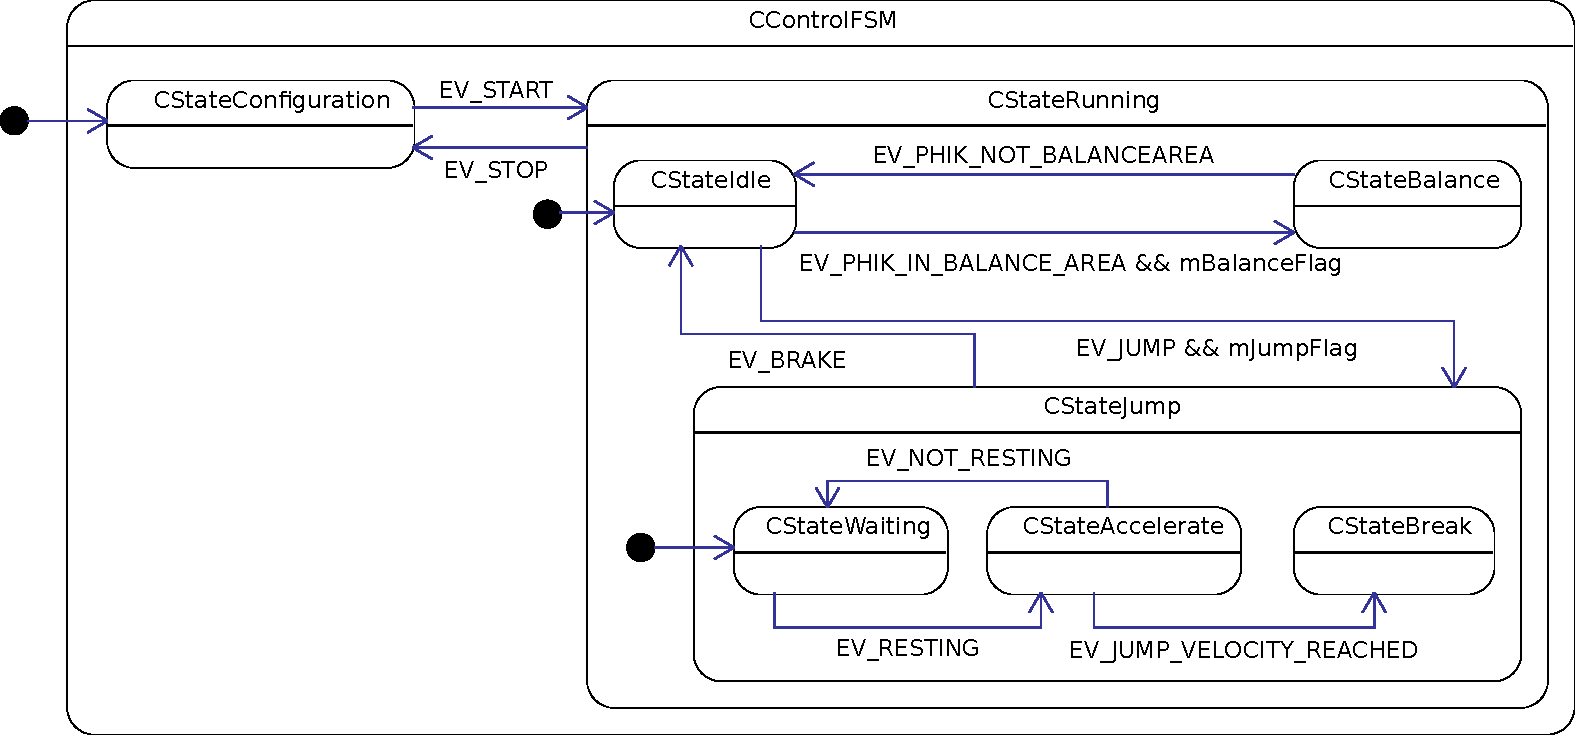
\includegraphics[width=\linewidth]{KontrollFSM}
	\caption{Zustandsdiagramm Kontrollkomponente, Quelle: eigene Darstellung}
\end{figure}

\newpage
Der Zustandsautomat wird nach \cite{WieTra} implementiert. Die Klasse  \textit{CFSM} dient als Basis für die Zustandsmaschine und die Oberzustände. Unterzustände hingegen werden als Methoden realisiert. Jeder Oberzustand verfügt außerdem über den Zustand \textit{CStateDefaultInitial}. Dieser dient als Dummyzustand, der angenommen wird wenn der Oberzustand verlassen wird. Bei Betreten des Oberzustandes wird ein internes \textit{EV\_INIT} Event generiert, welches den Übergang in den eigentlichen Startzustand veranlasst.

\begin{figure}[h]
	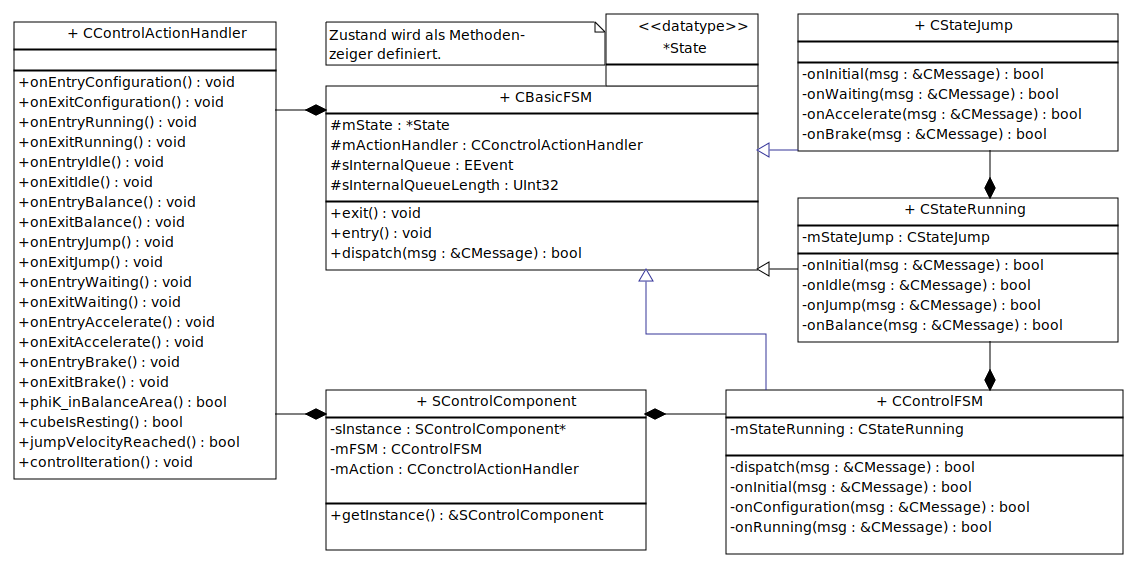
\includegraphics[width=\linewidth]{KontrollFSMKlassendiagra}
	\caption{Klassendiagramm Zustandsautomat, Quelle: eigene Darstellung}
\end{figure}

\subsection*{Aufgaben von \textit{CStateConfiguration}}
Der Zustand \textit{CStateConfiguration} ermöglicht die Einstellung der Steuereinheit. Einerseits kann die gewünschte Funktion durch Manipulieren der Flags \textit{mJumpFlag}, \textit{mBalanceFlag} und \textit{mTransmitFlag} eingestellt werden. Diese Flags werden von der Steuereinheit gespeichert und als Bedingungen an gewisse Zustandsübergänge gekoppelt. Dadurch kann das Aufspringen, das Balancieren um den Sollwert und die Übermittlung der physikalischen Zustandswerte ein- bzw. ausgeschaltet werden.
Zusätzliche können Parameter der Regelung konfiguriert werden. Einerseits kann die nötige Geschwindigkeit der Schwungmasse zum Aufspringen durch das Event \textit{EV\_SET\_JUMP\_VELOCITY} gesetzt werden. Andererseits können die Regelparameter konfiguriert werden. Die hierfür benötigten Events hängen von der verwendeten Reglerstruktur ab und können somit noch nicht endgültig festgelegt werden.

\begin{figure}[h]
	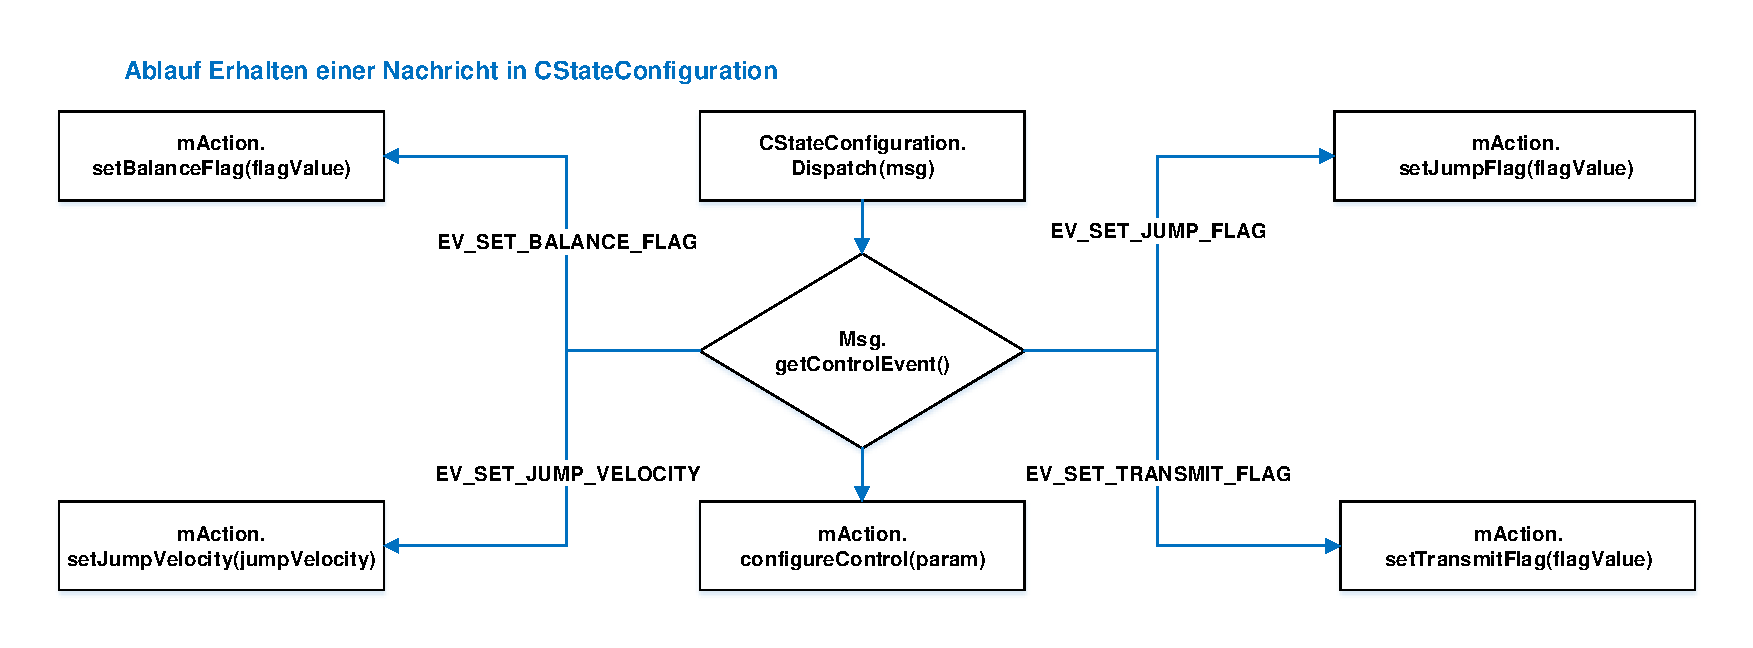
\includegraphics[width=\linewidth]{PAP_CStateConfiguration}
	\caption{Ablaufplan CStateConfiguration, Quelle: eigene Darstellung}
\end{figure}

\newpage
\subsection*{Aufgaben von \textit{CStateRunning}}
Die eigentliche Funktionalität der Steuerung steckt in dem Zustand \textit{CStateRunning}. Bei Betreten dieses Zustandes wird ein Softtimer gestartet, welcher zyklisch Events an die Komponente schickt. Dadurch wird die gewünschte Abtastrate der Regelung realisiert. Erhält die FSM ein solches Timerevent werden die folgenden Aktionen ausgeführt.

In dem Zustand \textit{CStateIdle} wird geprüft ob der Ausfallwinkel des Würfels sich im Regelungsbereich befindet. Gegebenenfalls wird das Event \textit{EV\_PHIK\_IN\_BALANCEAREA} in die interne Queue geschrieben.

In dem Zustand \textit{CStateBalance} wird ebenfalls geprüft ob der Würfel sich noch im Regelungsbereich befindet. Falls dies gegeben ist wird ein Regelungszyklus durchgeführt. Hat der Würfel den vorgegebenen Bereich verlassen wird das interne Event \textit{EV\_PHIK\_NOT\_BALANCEAREA} ausgelöst.

In dem Zustand \textit{CStateJump} wird nach dessen aktuellen Unterzustand entsprechend gehandelt. 
In dem Unterzustand \textit{CStateWaiting}  wird geprüft ob der Würfel die Ruhelage erreicht hat. Daraufhin wird das interne Event \textit{EV\_RESTING} und somit ein Wechsel in \textit{CStateAccelerate} ausgelöst. 

In dem Unterzustand \textit{CStateAccelerate} wird ebenfalls die Ruhelage geprüft. Hat der Würfel diese verlassen so wird das interne Event \textit{EV\_NOT\_RESTING} ausgelöst, woraufhin wieder in \textit{CStateWaiting} gewechselt wird. Bleibt die Ruhelage erhalten wird geprüft ob die Schwungmasse die erforderliche Geschwindigkeit zum Aufrichten erreicht hat. Ist dies der Fall wird das interne Event \textit{EV\_JUMP\_VELOCITY\_REACHED} ausgelöst, welches den Übergang in \textit{CStateBrake}. 


In dem Unterzustand \textit{CStateBrake} wird der Bremsvorgang überwacht. Bei Betreten des Zustandes wird die Bremse aktiviert und anschließend geprüft ob die Schwungmasse zur Ruhe gekommen ist. Daraufhin wird das interne Event \textit{EV\_BRAKE} ausgelöst, welches zum Verlassen des Zustandes \textit{CStateJump} und somit zum deaktivieren der Bremse führt.

\begin{figure}[h]
	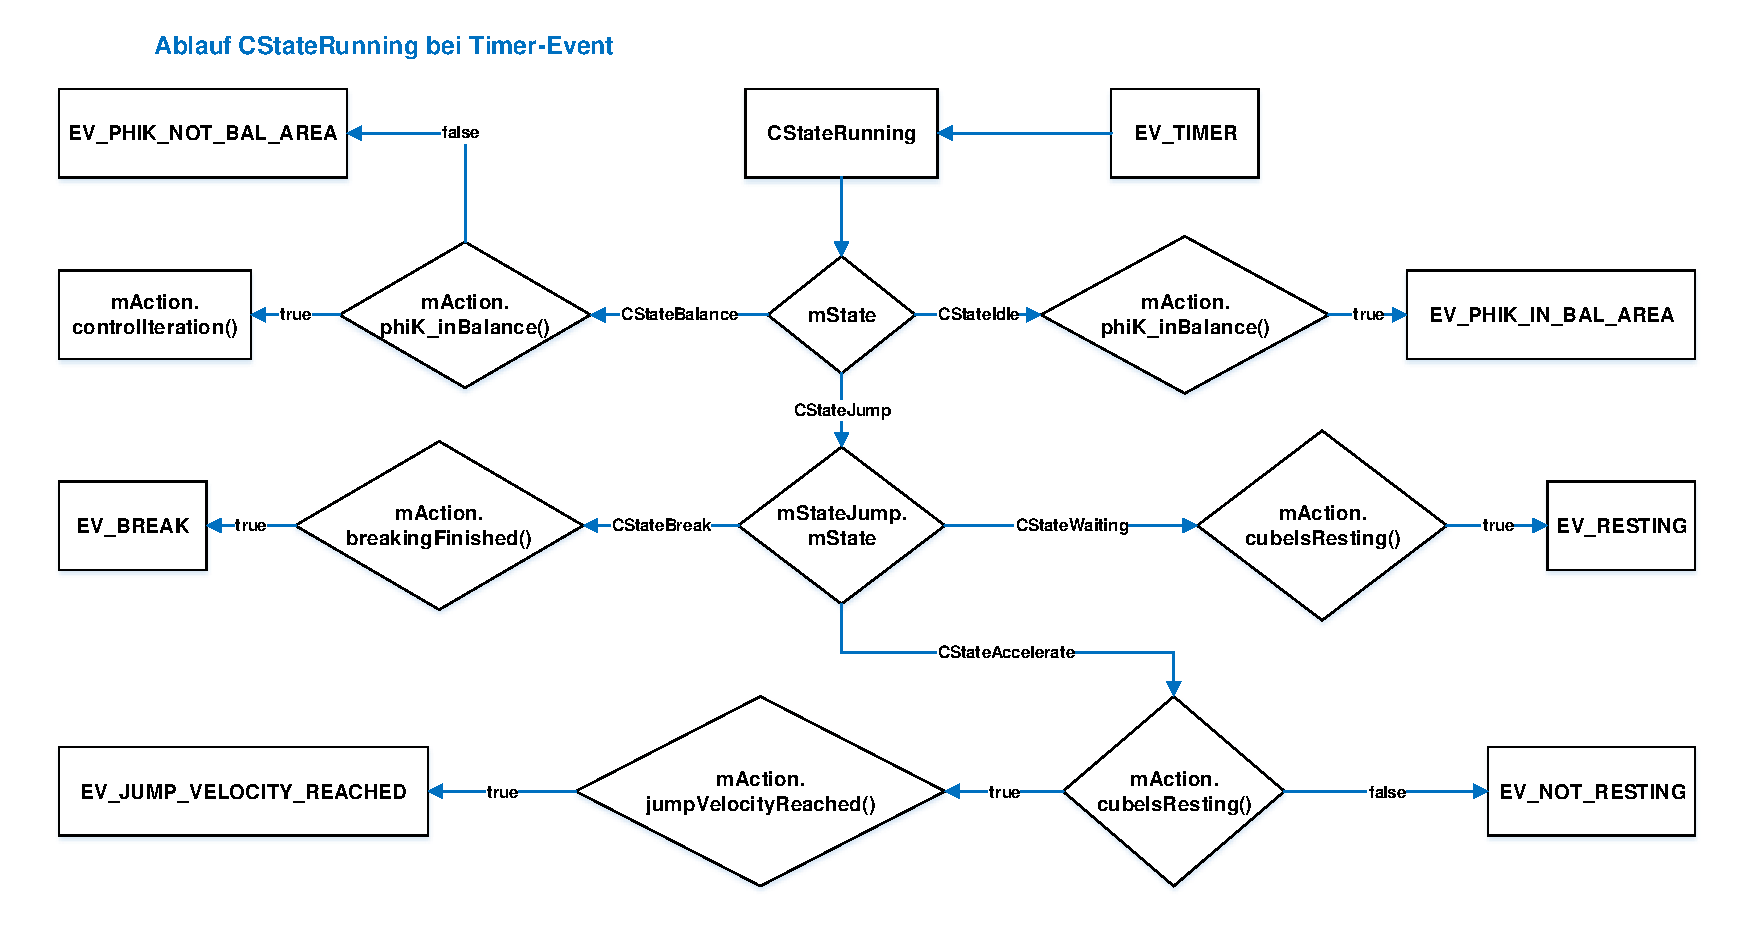
\includegraphics[width=\linewidth]{PAP_CStateRunning}
	\caption{Ablaufplan CStateRunning, Quelle: eigene Darstellung}
\end{figure}


\newpage
\subsection*{Aktionen von \textit{CControlActionHandler}}
Die auszuführenden Aktionen werden in der Klasse \textit{CControlActionHandler} gekapselt. Es werden Methoden für Aktionen bei Betreten und Verlassen von Zuständen implementiert. Auf Übergangsfunktionen wird (vorläufig) verzichtet. Außerdem werden weitere Hilfsmethoden eingeführt, welche Aktionen auslösen die nicht an Zustandsübergänge gekoppelt sind.

Hierfür verfügt die Klasse über Instanzen des Reglers und der Klassen zur Hardwareansteuerung. Zusätzlich hält er eine Referenz auf \textit{SSoftTimer} um diesen zu starten bzw. zu stoppen. Die oben angesprochenen Flags zur Kontrolle der Funktionalität werden ebenfalls von \textit{CControlActionHandler} verwaltet.

\begin{figure}[h]
	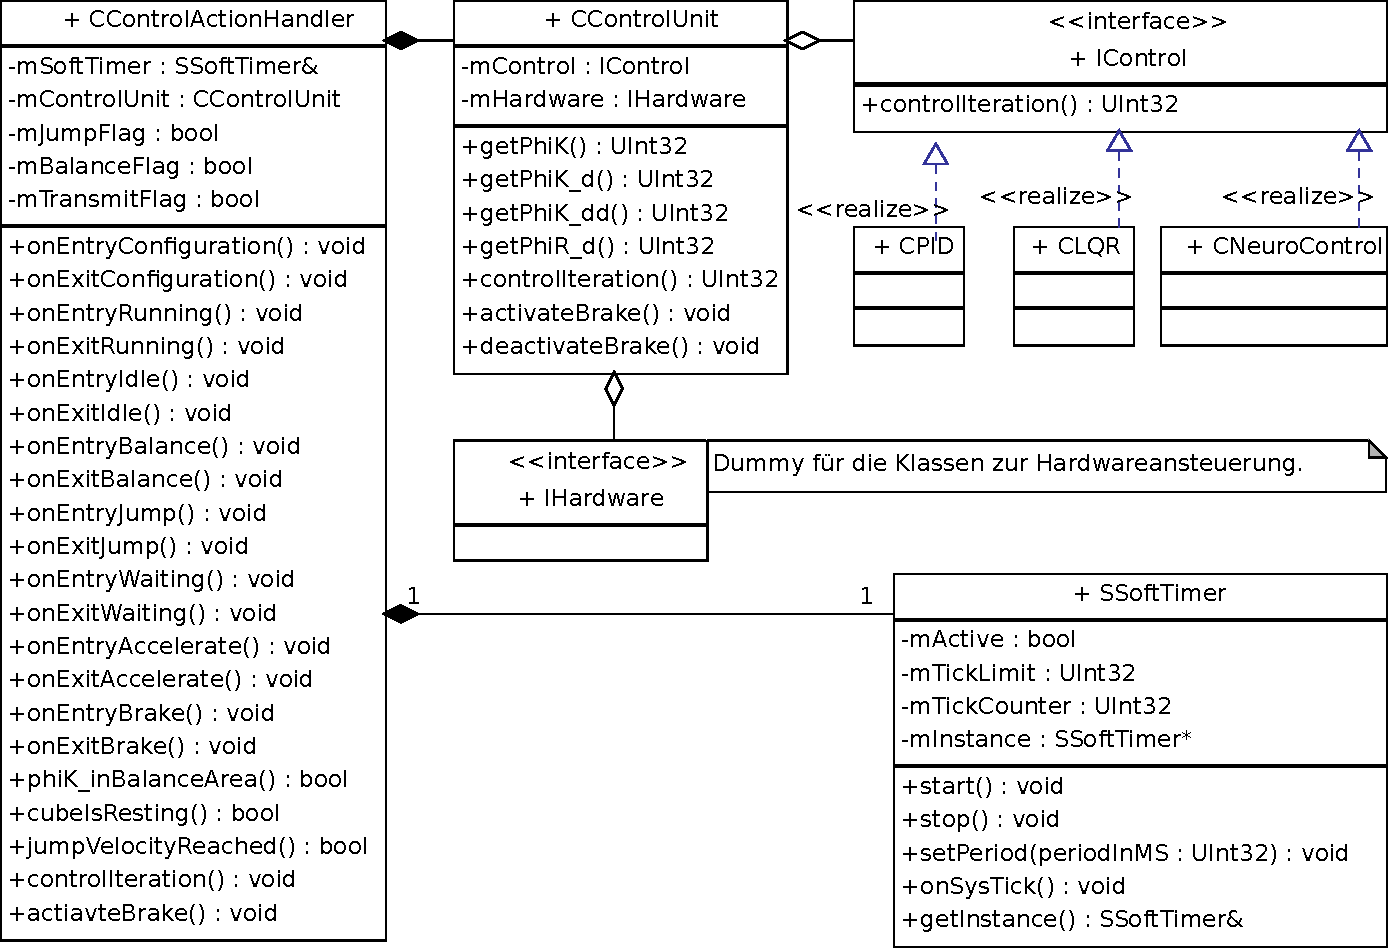
\includegraphics[width=\linewidth]{ControlActionHandler}
	\caption{Klassendiagramm ControlActionHandler, Quelle: eigene Darstellung}
\end{figure}

Der Softtimer wird an den SysTimer gekoppelt, bei erreichen des Zählerlimit wird das Event \textit{EV\_TIMER} ausgelöst. Dadurch wird die periodische Abtastung des Regelsystem sicher gestellt.
Mit Hilfe der Klassen zur Hardwareansteuerung können die Sensorwerte abgefragt und ausgewertet werden. Bei Bedarf werden entsprechende Events generiert, welche wiederum Zustandsübergänge zur Folge haben.

\newpage
Die einzelnen folgende Tabelle zeigt die Methoden von \textit{CControlActionHandler} und deren Aktionen. Aus Gründen der Übersicht und Einheitlichkeit werden auch Methoden ohne Aufgabe implementiert bzw. aufgerufen.
\begin{table}[h]
\centering
\label{my-label}
\begin{tabular}{|l|l|}
\hline
\textbf{Methode von CControlAction} & \textbf{Auszuführende Aktion}               \\ \hline
void onEntryConfiguration()         & -                                           \\ \hline
void onExitConfiguration()          & -                                           \\ \hline
void onEntryRunning()               & Softtimer starten                           \\ \hline
void onExitRunning()                & Softtimer stoppen                           \\ \hline
void onEntryIdle()                  & Softtimerfrequenz anpassen                  \\ \hline
void onExitIdle()                   & -                                           \\ \hline
void onEntryBalance()               & Softtimerfrequenz anpassen                  \\ \hline
void onExitBalance()                & -                                           \\ \hline
void onEntryJump()                  & Softtimerfrequenz anpassen                  \\ \hline
void onExitJump()                   & Prüfen ob Bremse deaktiviert ist            \\ \hline
void onEntyWaiting()                & -                                           \\ \hline
void onExitWaiting()                & -                                           \\ \hline
void onEntryAccelerate()            & Motormoment setzen                          \\ \hline
void onExitAccelerate()             & Motor stoppen                               \\ \hline
void onEntryBrake()                 & Bremse aktivieren                           \\ \hline
void onExitBrake()                  & Bremse deaktivieren                         \\ \hline
bool phiK\_inBalanceArea()          & Prüft ob der Würfel im Regelbereich         \\ \hline
bool cubeIsResting()                & Prüft ob der Würfel in Ruhelage             \\ \hline
bool jumpVelocityReached()          & Prüft ob die Sprunggeschwindigkeit erreicht \\ \hline
void controlIteration()             & Führt einen Regelzyklus aus                 \\ \hline
\end{tabular}
\end{table}


\newpage
\section{Aufbau der Kommunikationskomponente}
Die Aufgabe der Kommunikationskomponente besteht darin einerseits Befehle der Bedieneinheit anzunehmen und andererseits aktuelle Systeminformationen zu übermitteln. Die Übertragung der Daten erfolgt mittels Bluetooth und dem Serial Port Profile. Zur Ansteuerung des Bluetooth Modul wird eine serielle Schnittstelle verwendet. Folglich müssen deren Interrupts verarbeitet werden und die einzelnen Byte zu Informationspaketen zusammengesetzt werden. 
Die Komponente verfügt über einen Puffer, der empfangene Datenpakete enthält. Diese müssen von der Kommunikationseinheit in Nachrichten übersetzt werden. Der zweite Puffer speichert Nachrichten, welche in Form von Datenpaketen an die Bedieneinheit übermittelt werden müssen.

\begin{figure}[h]
	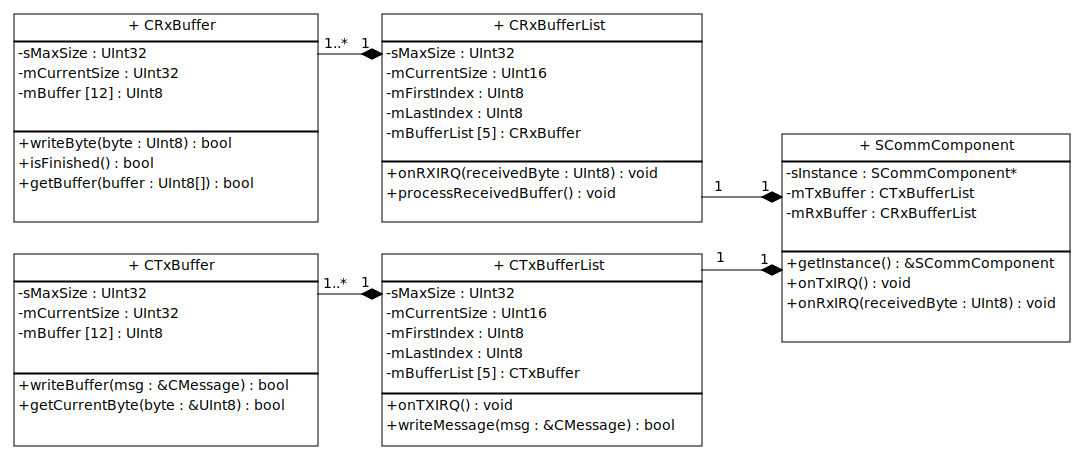
\includegraphics[width=\linewidth]{CommBuffer}
	\caption{Klassendiagramm Comm-Komponente, Quelle: eigene Darstellung}
\end{figure}

\subsection*{Aufbau der Bluetoothpakete}
Der Datenaustausch zwischen Würfel und Bedieneinheit erfolgt byteweise. Die einzelnen Bytes werden zu logischen Paketen zusammen gesetzt. Alle Pakete besitzen eine fixe, einheitliche Größe von 6 Bytes. Das erste Byte enthält die die ID des Empfängers, im zweiten Byte dient zur Speicherung des Ereignis bzw. Befehls. Die übrigen vier Bytes sind für zusätzliche Nutzdaten,wie z.B. Sensorwerte reserviert.

Der Inhalt eines empfangenen Paket wird durch entsprechenden Proxyaufruf in eine Nachricht umgesetzt. Der Aufbau der einzelnen Pakete wird in einer Tabelle dokumentiert, hierbei ist darauf zu achten bei Werten, die größer als ein Byte sind die Position des MSB und LSB zu notieren.


\begin{landscape}

\begin{table}[]
\centering
\caption{Aufbau der Datenpakete}
\label{my-label}
\begin{tabular}{|l|l|l|l|l|l|l|}
\hline
\textbf{Byte0} & \textbf{Byte1}                  & \textbf{Byte2}      & \textbf{Byte3} & \textbf{Byte4} & \textbf{Byte5} & \textbf{Anmerkung}   \\ \hline
CONTROL\_COMP  & EV\_START                       &                     &                &                &                &                      \\ \hline
CONTROL\_COMP  & EV\_STOP                        &                     &                &                &                &                      \\ \hline
CONTROL\_COMP  & EV\_SET\_JUMP\_FLAG             & flagValue           &                &                &                &                      \\ \hline
CONTROL\_COMP  & EV\_SET\_BALANCE\_FLAG          & flagValue           &                &                &                &                      \\ \hline
CONTROL\_COMP  & EV\_SET\_TRANSMIT\_FLAG         & flagValue           &                &                &                &                      \\ \hline
CONTROL\_COMP  & EV\_JUMP                        &                     &                &                &                &                      \\ \hline
CONTROL\_COMP  & EV\_SET\_PID\_P\_VALUE          & P\_Value(LSB)       & P\_Value       & P\_Value       & P\_Value(MSB)  & float                \\ \hline
CONTROL\_COMP  & EV\_SET\_PID\_I\_VALUE          & I\_Value(LSB)       & I\_Value       & I\_Value       & I\_Value(MSB)  & float                \\ \hline
CONTROL\_COMP  & EV\_SET\_PID\_D\_VALUE          & D\_Vaue(LSB)        & D\_Value       & D\_Value       & D\_Value(MSB)  & float                \\ \hline
CONTROL\_COMP  & EV\_SET\_JUMP\_VELOCITY         & velocity(LSB)       & velocity       & velocity       & velocity(MSB)  & SI-Einheit als float \\ \hline
               &                                 &                     &                &                &                &                      \\ \hline
COMM\_COMP     & EV\_TRANSMIT\_TORQUE            & Torque(LSB)         & Torque         & Torque         & Torque(MSB)    & SI-Einheit als float \\ \hline
COMM\_COMP     & EV\_TRANSMIT\_PHI\_K            & PhiK(LSB)           & PhiK           & PhiK           & PhiK(MSB)      & SI-Einheit als float \\ \hline
COMM\_COMP     & EV\_TRANSMIT\_PHI\_K\_D         & PhiK\_d(LSB)        & PhiK\_d        & PhiK\_d        & PhiK\_d(MSB)   & SI-Einheit als float \\ \hline
COMM\_COMP     & EV\_TRANSMIT\_PHI\_K\_DD        & PhiK\_dd(LSB)       & PhiK\_dd       & PhiK\_dd       & PhiK\_dd(MSB)  & SI-Einheit als float \\ \hline
COMM\_COMP     & EV\_TRANSMIT\_BRAKE\_STATE      & brakeState          &                &                &                &                      \\ \hline
COMM\_COMP     & EV\_TRANSMIT\_FSM\_STATE\_ENTRY & enteredState        &                &                &                &                      \\ \hline
COMM\_COMP     & EV\_TRANSMIT\_UNHANDELD\_EV     & unhandeledControlEV &                &                &                &                      \\ \hline
COMM\_COMP     & EV\_HARDWARE\_ERROR             & hardwareID          &                &                &                &                      \\ \hline
\end{tabular}
\end{table}

\end{landscape}

\newpage
\subsection*{Funktionsablauf des RX-Puffer}
Falls ein RX-Interrupt anliegt wird zuerst geprüft ob der Puffer voll ist. Ggf. wird ein entsprechendes Fehler-Event erzeugt. Ansonsten wird das empfangene Byte in den aktuellen Puffer geschrieben. Falls dieses Datenpaket voll ist, wird das Event \textit{EV\_COM\_RECEIVED} ausgelöst, welches die Verarbeitung des Datenpaket veranlasst.

Bei der Verarbeitung des Event \textit{EV\_COM\_RECEIVED}  wird zuerst geprüft ob ein Datenpaket vorhanden ist. Ggf. wir das erste Paket aus der FIFO-Liste entnommen und über den Proxy eine entsprechende Nachricht erzeugt.

\begin{figure}[h]
	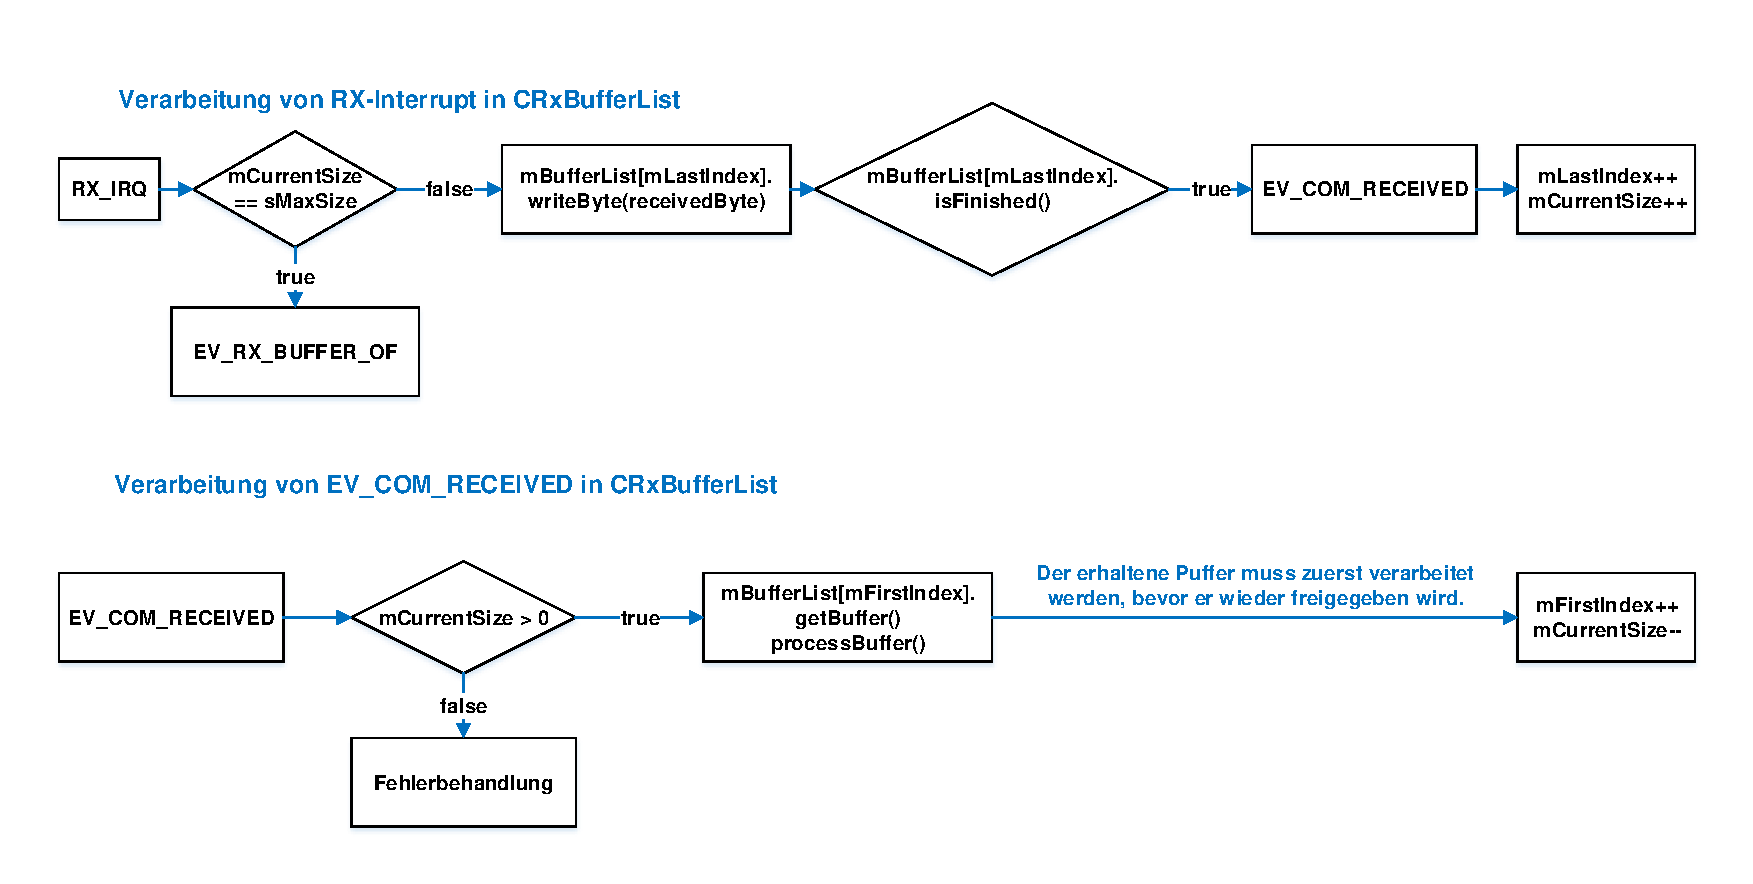
\includegraphics[width=\linewidth]{PAP_RxPuffer}
	\caption{Ablaufplan RX-Puffer, Quelle: eigene Darstellung}
\end{figure}

\subsection*{Funktionsablauf des TX-Puffer}
Die Nachrichtenvermittlung an die Bedieneinheit verläuft nach dem gleichen Prinzip. Bei dem Erhalten des Event \textit{EV\_TRANSMIT\_MSG} wird geprüft ob der Puffer voll ist. Ggf. wird ein Fehlerevent produziert. Trifft dies nicht zu wird der Nachrichteninhalt in einen freien Datenpuffer geschrieben und der TX-Interrupt aktiviert.

Tritt ein TX-Interrupt auf wird ein Byte aus dem aktuellen Datenpuffer übermittelt. Anschließend wird geprüft ob der Datenpuffer vollständig übermittelt wurde. Ggf. wir dieser wieder freigegeben und falls keine weiteren Daten übermittelt werden müssen, wird der TX-Interrupt deaktiviert.

\begin{figure}[h]
	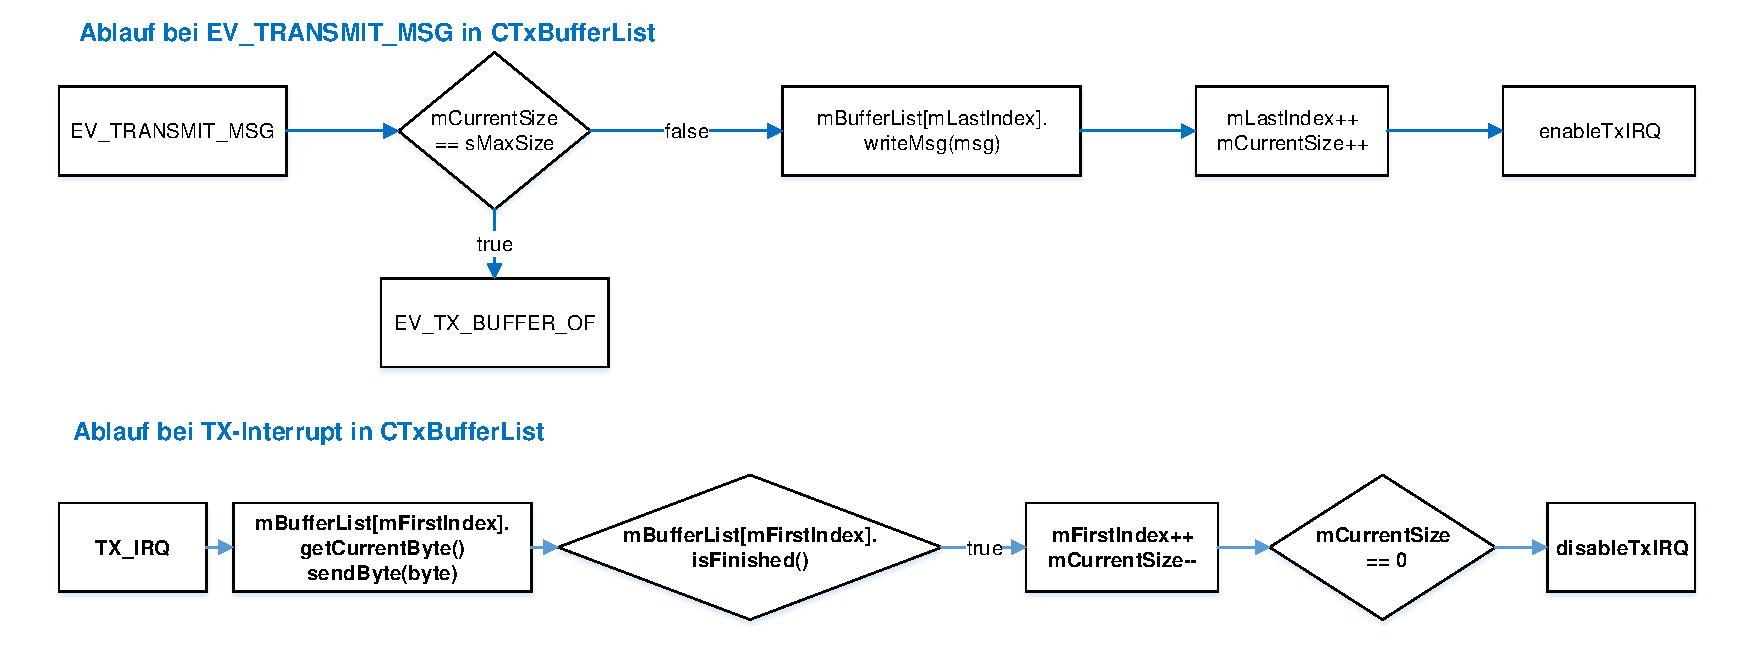
\includegraphics[width=\linewidth]{PAP_TxPuffer}
	\caption{Ablaufplan TX-Puffer, Quelle: eigene Darstellung}
\end{figure}

\newpage
\section{Implementation des Reglers}
In diesem Abschnitt wird die Umsetzung der Regler in Software erläutert. Die Regler benötigen als Eingangsgröße den Zustandsvektor $x$. Dieser besteht aus den Größen $\phi_K$, $\dot{\phi_K}$ und $\dot{\phi_R}$. Außerdem muss die Winkelbeschleunigung $\ddot{\phi_K}$ zu Analysezwecken aufgezeichnet werden. Der Ausfallwinkel des Körpers und dessen zwei Ableitungen werden mit Hilfe von einem Magnetometer, Gyrometer und Beschleunigungssensor aufgenommen. Diese drei Sensoren sind auf einem IC verbaut und können über I2C angesteuert werden. Die aktuellen Sensorwerte werden als 16-Bit Ganzzahlen übergeben (signed unsigned?). Dem Datenblatt kann der einheitenbehaftete Faktor zur Umrechnung in die physikalische Größe entnommen werden.

\subsection{Berechnung der Winkelbeschleunigung $\ddot{\phi_K}$}
Der Dreiachs-Beschleunigungssensor gibt die Beschleunigung in x- und y-Richtung wieder. Daraus wird die Tangentialbeschleunigung des Sensors berechnet. Über den Abstand des Sensors zum Drehpunkt kann daraufhin die Winkelbeschleunigung des Körpers berechnet werden.

\[\ a_t := Tangentialbeschleunigung des Sensors \]
\[\ r_AS := Abstand des Sensors zum Drehpunkt \]
\[\ \ddot{x} := Beschleunigung in x-Richtung in \frac{m}{s} \]
\[\ \ddot{y} := Beschleunigung in y-Richtung in \frac{m}{s} \]
\[\ a_t = \sqrt{\ddot{x}^2 + \ddot{y}^2} \]
\[\ \ddot{\phi_K} = \frac{a_t}{r_AS} \] 

\subsection{Berechnung der Winkelgeschwindigkeit $\dot{\phi_K}$}
Der Gyrosensor gibt die Winkelbeschleunigung in Grad pro Sekunde wieder. Dementsprechend einfach kann die Umrechnung in SI-Einheiten durchgeführt werden.

\[ \dot{\phi_{K,S}} := Winkelgeschwindigkeit in Grad pro Sekunde \]
\[\ \dot{\phi_K} = \frac{2*\pi}{360} \cdot \dot{\phi_{K,S}} \]

\subsection{Berechnung des Ausfallwinkels $\phi_K$}
Der Ausfallwinkel des Körpers wird mit Hilfe eines Magnetometer bestimmt. Über die I2C versendet der Sensor die magnetische Flussdichte in x- und y-Richtung. Daraus wird der Winkel des Sensor und somit des Körpers berechnet.

ATan von x und y gibt den Winkel, wenn richtig kalibriert kann das sogar funktionieren, ausprobieren mit arduino oder so

\newpage
\section{Testen der Software}
Die Software muss geprüft werden um den problemlosen Einsatz zu garantieren. Hierbei muss zwischen den Hardwareansteuerung, der Validierung des Reglers und der Komponentenstruktur bzw. Logik unterschieden werden.
Die Softwareteile zur Ansteuerung der Hardware muss einzeln geprüft werden bevor sie in das Gesamtsystem eingehängt werden. Diese Tests erfolgen sowohl manuell als auch automatisch.

Die Validierung des Reglers erfordert einerseits die Prüfung der Implementierung. D.h. der Regler muss den Eingangsgrößen entsprechende Werte generieren. Andererseits muss der verwendete Regler mit den Anforderungen an den Regelkreis abgeglichen werden. Hierzu wird das \textit{mTransmitFlag} der Regelkomponente aktiviert. Daraufhin werden alle Sensor- und Reglerwerte an die Bedieneinheit übermittelt. Folglich kann die Überprüfung der oben genannten Kriterien vollautomatisch durchgeführt werden.

Die Prüfkriterien der Komponentenstruktur beinhalten die Erzeugung von Nachrichten und deren Verteilung, die Kodierung und Dekodierung von Kommunikationspaketen sowie die Zustandsübergänge und deren Folgeaktionen. Bei entsprechender Einstellung überträgt die Kontrollkomponente ihren aktuellen Zustand an die Bedieneinheit. Zusätzlich wird die Ansteuerung der Sensoren durch eine serielle Schnittstelle ersetzt. Somit können Blackbox-Tests vollautomatisch durchgeführt werden. Auftretende Fehler müssen manuell per Debugger zurückverfolgt werden.


\subsection*{Reglerersatz für Softwaretests}
Um die Komponentenarchitektur, deren Nachrichtenstruktur und die Logik der Zustandsmaschine zu testen, wird der Regler und die Sensorik durch eine serielle Schnittstelle ersetzt. Somit ist es möglich automatisiert beliebige Prüfabläufe durchzuführen und die Softwarefunktionalität gezielt zu überprüfen.

\begin{table}[h]
\centering
\label{my-label}
\begin{tabular}{|l|l|l|l|l|}
\hline
\textbf{CuBa-Anfrage} & \textbf{}   & \textbf{}   & \textbf{Rx-Reaktion} &               \\ \hline
REQUEST\_PHI\_K       &             &             & phiK(LSB)            & phiK(MSB)     \\ \hline
REQUEST\_PHI\_K\_D    &             &             & phiK\_d(LSB)         & phiK\_d(MSB)  \\ \hline
REQUEST\_PHI\_K\_DD   &             &             & phiK\_dd(LSB)        & phiK\_dd(MSB) \\ \hline
REQUEST\_PHI\_R\_D    &             &             & phiR\_d(LSB)         &  phiR\_d(MSB) \\ \hline
SET\_MOTOR\_TORQUE    & Torque(LSB) & Torque(MSB) &                      &               \\ \hline
SET\_BRAKE\_STATE     & brakeState  &             &                      &               \\ \hline
\end{tabular}
\end{table}

\newpage
\begin{thebibliography}{\hspace{0.5cm}}
	\bibitem[WieTra]{WieTra} Joachim Wietzke, Manh Tien Tran: Automotive Embedded Systeme
	\bibitem[Bar]{Bar} Richard Barry: Using the FreeRTOS Real Time Kernel - A Practical Guide
\end{thebibliography}

\end{document}